\documentclass[border=10pt]{standalone}
\usepackage[svgnames]{xcolor}
\usepackage{amsmath}
\usepackage{pgfplots}
\pgfplotsset{compat=newest}
\usepackage[sfdefault]{FiraSans}
\usepackage{FiraMono}
\renewcommand*\familydefault{\sfdefault}
\begin{document}
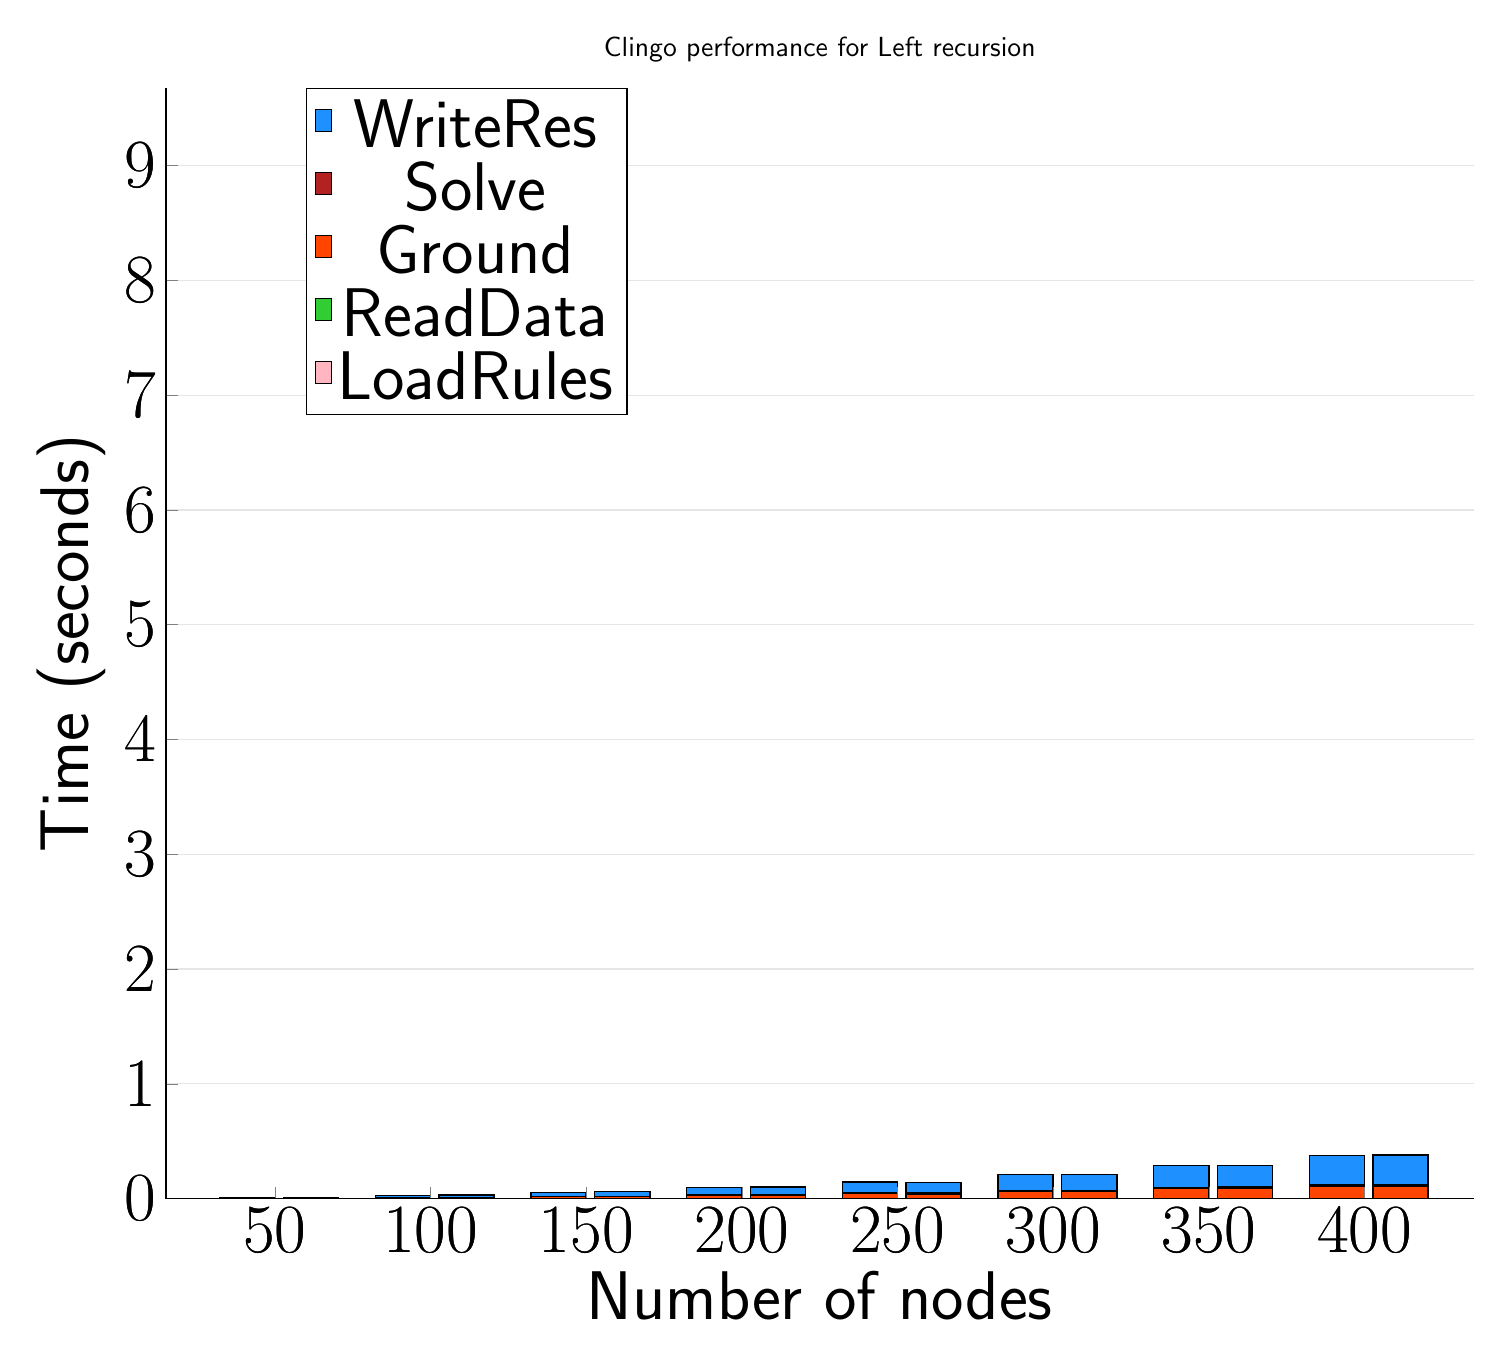
\begin{tikzpicture}
\begin{axis}[
   ybar stacked,
   title={Clingo performance for Left recursion},
   bar shift=-10pt,
   width=1.5\textwidth,
   bar width=0.7cm,
   ymajorgrids, tick align=inside,
   major grid style={draw=gray!20},
   xtick=data,
   ymin=0, ymax=9.677999997138977,
   axis x line*=bottom,
   axis y line*=left,
   enlarge x limits=0.1,
   legend style={
       at={(0.23, 1)},
       anchor=north,
       legend columns=1,
       font=\Huge,
   },
   ylabel={Time (seconds)},
   xlabel={Number of nodes},
   label style={font=\Huge},
   tick label style={font=\Huge},
]
\addlegendimage{fill=DodgerBlue, draw=black, line width=0.2pt}
\addlegendentry{WriteRes}
\addlegendimage{fill=FireBrick, draw=black, line width=0.2pt}
\addlegendentry{Solve}
\addlegendimage{fill=OrangeRed, draw=black, line width=0.2pt}
\addlegendentry{Ground}
\addlegendimage{fill=LimeGreen, draw=black, line width=0.2pt}
\addlegendentry{ReadData}
\addlegendimage{fill=LightPink, draw=black, line width=0.2pt}
\addlegendentry{LoadRules}
\addplot +[fill=LightPink, draw=black, line width=0.5pt] coordinates {
    (50, 0.0009999990463256836)
    (100, 0.0)
    (150, 0.0)
    (200, 0.0)
    (250, 0.0)
    (300, 0.0)
    (350, 0.0)
    (400, 0.0)
};
\addplot +[fill=LimeGreen, draw=black, line width=0.5pt] coordinates {
    (50, 0.0)
    (100, 0.0009999990463256836)
    (150, 0.0019999980926513673)
    (200, 0.0009999990463256836)
    (250, 0.0)
    (300, 0.0)
    (350, 0.0009999990463256836)
    (400, 0.0)
};
\addplot +[fill=OrangeRed, draw=black, line width=0.5pt] coordinates {
    (50, 0.0029999971389770507)
    (100, 0.005999994277954101)
    (150, 0.014999985694885254)
    (200, 0.02799999713897705)
    (250, 0.04499998092651367)
    (300, 0.06100001335144043)
    (350, 0.08600001335144043)
    (400, 0.10999999046325684)
};
\addplot +[fill=FireBrick, draw=black, line width=0.5pt] coordinates {
    (50, 0.0)
    (100, 0.0)
    (150, 0.0019999980926513673)
    (200, 0.0019999980926513673)
    (250, 0.0039999961853027345)
    (300, 0.007999992370605469)
    (350, 0.01100001335144043)
    (400, 0.01399998664855957)
};
\addplot +[fill=DodgerBlue, draw=black, line width=0.5pt] coordinates {
    (50, 0.0039999961853027345)
    (100, 0.017999982833862303)
    (150, 0.03600001335144043)
    (200, 0.06500000953674316)
    (250, 0.09700000286102295)
    (300, 0.13999998569488525)
    (350, 0.18999998569488524)
    (400, 0.2530000448226929)
};
\end{axis}
\begin{axis}[
   ybar stacked,
   bar shift=13pt,
   width=1.5\textwidth,
   bar width=0.7cm,
   ymajorgrids, tick align=inside,
   major grid style={draw=none},
   xtick=data,
   ymin=0, ymax=9.677999997138977,
   axis x line*=none,
   axis y line*=none,
   enlarge x limits=0.1,
   label style={font=\Huge},
   tick label style={font=\Huge},
]
\addplot +[fill=LightPink, draw=black, line width=0.5pt] coordinates {
    (50, 0.0)
    (100, 0.0)
    (150, 0.0)
    (200, 0.0)
    (250, 0.0)
    (300, 0.0)
    (350, 0.0)
    (400, 0.0)
};
\addplot +[fill=LimeGreen, draw=black, line width=0.5pt] coordinates {
    (50, 0.0)
    (100, 0.0)
    (150, 0.0)
    (200, 0.0)
    (250, 0.0)
    (300, 0.0)
    (350, 0.0)
    (400, 0.0)
};
\addplot +[fill=OrangeRed, draw=black, line width=0.5pt] coordinates {
    (50, 0.0)
    (100, 0.009999999999999997)
    (150, 0.019999999999999997)
    (200, 0.030000000000000006)
    (250, 0.03999999999999999)
    (300, 0.06100000000000001)
    (350, 0.08899999999999998)
    (400, 0.11000000000000001)
};
\addplot +[fill=FireBrick, draw=black, line width=0.5pt] coordinates {
    (50, 0.0)
    (100, 0.0)
    (150, 0.0)
    (200, 0.0)
    (250, 0.010000000000000009)
    (300, 0.008999999999999996)
    (350, 0.010999999999999994)
    (400, 0.010000000000000009)
};
\addplot +[fill=DodgerBlue, draw=black, line width=0.5pt] coordinates {
    (50, 0.009999999999999997)
    (100, 0.020000000000000007)
    (150, 0.03899999999999999)
    (200, 0.06999999999999998)
    (250, 0.08999999999999998)
    (300, 0.139)
    (350, 0.18899999999999997)
    (400, 0.261)
};
\end{axis}
\end{tikzpicture}

\end{document}
